\section{考虑频偏消除的成像仿真}
\subsection{CSI频偏模型}
在实际的通信系统中,测量得到的CSI会受到多径效应,收发机的不同步处理,以及软/硬件上存在的客观误差等因素的
影响,导致受到频偏的影响。最主要的频偏影响因素有:采样频率偏移(SFO: Sampling Frequency Offset),以及
包检测误差(PDD: Packet Detection Delay)以及载波频率偏移(CFO: Carrier Frequency Offset)等\cite{ma2019wifi}\cite{Precise_PDP_WiFi}。
受以上因素影响的接收信号(CSI)$\tilde{\boldsymbol{y}}$将满足如下表达式\cite{zhang2022practical}:
\begin{align}
  \tilde{\boldsymbol{y}} &= \boldsymbol{y}e^{-j\theta_{\text{offset}}(t)} \nonumber 
  \\ &= \boldsymbol{y}e^{-j \left\{2\pi f[\theta_{\text{SFO}}(t)+\theta_{\text{PDD}}(t)]+2\pi \theta_{\text{CFO}}(t)\right\}}
  \text{。}
\end{align}
本文考虑的两种频偏情形:
\begin{enumerate}
  \item (类似SAR的情形)这种频偏的情形与我们后续实测时利用轨道移动模拟天线阵列一致,信号到达阵列上每一个点的频偏不一致。
  \begin{align}
    & \text{(情形一)}\quad \tilde{\boldsymbol{y}} = \boldsymbol{y}e^{-j\theta_{\text{offset}}} \nonumber \\
    &= \boldsymbol{y} \odot \left[e^{-j\left\{-j2\pi f[\theta_{\text{SFO},1}+\theta_{\text{PDD},1}]+2\pi \theta_{\text{CFO},1}\right\}},\cdots,e^{-j\left\{-j2\pi f[\theta_{\text{SFO},N}+\theta_{\text{PDD},N}]+2\pi \theta_{\text{CFO},N}\right\}}\right]
    \text{。}
    \label{情形一}
  \end{align}
  这里$\odot$指的是矩阵的点乘。
  \item (类似图~\ref{系统模型}一个巨大的接收阵列的情形)当然,我们考虑信号同时到达我们的天线阵列(考虑某一时刻的CSI),则有:
  \begin{align}
    \text{(情形二)}\quad
    \tilde{\boldsymbol{y}} = \boldsymbol{y}e^{-j\{2\pi f[\theta_{\text{SFO}}+\theta_{\text{PDD}}]+2\pi\theta_{\text{CFO}}\}}
    \text{。}
    \label{情形二}
  \end{align}
\end{enumerate}


如果不消除频偏,由于我们主要根据相位匹配滤波,会导致成像的某些径的峰值不够明显,各个目标成像峰值差距过大,成像模糊以及成像模糊等问题
(具体的仿真结果将与本文频偏消除后的结果,共同于小节~3.4介绍)。
\subsection{CSI频偏消除的方法}
目前主流的CSI频偏消除的方式主要有两种类型\cite{ma2019wifi}:
\begin{enumerate}
  \item 基于相位相位``相减''的方式\cite{wu2021wifi}。
  \begin{itemize}
    \item 两路CSI信号共轭相乘。
    \begin{align}
      \tilde{\boldsymbol{y}_1}\times\tilde{\boldsymbol{y}_2}^H = (\boldsymbol{y}_1e^{-j\theta_{\text{offset}}})\times(\boldsymbol{y}_2e^{-j\theta_{\text{offset}}})^H
      \text{,}
    \end{align}
    \item 两路CSI信号相除。
    \begin{align}
      \tilde{\boldsymbol{y}_1}/\tilde{\boldsymbol{y}_2} = (\boldsymbol{y}_1e^{-j\theta_{\text{offset}}})/(\boldsymbol{y}_2e^{-j\theta_{\text{offset}}})
      \text{。}
    \end{align}
  \end{itemize}
  \item 基于线性拟合的方法。
  \begin{itemize}
    \item 文章SignFi\cite{SignFi}提出了一种沿着CSI子载波与天线维度最小化拟合误差的方法:
    \begin{align}
      \rho^*, \beta^* = \arg \limits_{\rho,\beta} \min \sum_{r,f}(\Theta_{r,f} + 2\pi f \rho + \beta)^2
      \text{,}
    \end{align}
    这里,$\Theta_{r,f}$是测量得到的CSI相位,$\rho$与$\beta$是拟合的参数。如果拟合完美,我们可以近似的得到:
    $\rho^* = \theta_{\text{SFO}} + \theta_{\text{PDD}}$以及$\beta^*/(2\pi) = \theta_{\text{CFO}}$。
  \end{itemize}
\end{enumerate}


为了简单考虑,本文后续主要考虑了基于两路CSI信号共轭相乘的方式消除频偏。仿真结果在小节~3.4介绍。
\subsection{结合CSI共轭相乘和PARAFAC算法的频偏消除成像}
直接利用两路CSI信号共轭相乘,然后对多径信号直接成像的操作并不完美,主要体现在:
\begin{enumerate}
  \item 对于接收两路CSI的天线,要求一个较大的天线间距。
  \item 对于某些目标,峰值不够明显,甚至无法被检测到。
\end{enumerate}

为了克服以上问题,将多径信号分离出来,再对每一条多径分别消除频偏并成像是一个可行的方案。
本小节基于平行因子分析(PARAFAC,Parallel Factor)中的TPF (Trilinear Parallel Factor)
技术中的复平行因子分析算法(COMFAC, Complex parallel Factor Analysis)\cite{bro1999fast},估计接收信号
的每一条径的CSI\cite{TPF}。之后对每一条径的CSI分别做共轭相乘操作以消除频偏,并分别成像。


目前所采用的TPF估计原理如下:
\begin{itemize}
  \item 假设在某一时刻,有两路(带有频偏的)接收信号$\widetilde{\boldsymbol{y}_1},\widetilde{\boldsymbol{y}_2} \in \mathbb{C}^{F\times N}$,这里$F$为子载波数目,
  $N$为接收天线的数目。
  \item 将以二维的CSI转化为三维矩阵的形式$\widetilde{\boldsymbol{Y}}_1,\widetilde{\boldsymbol{Y}}_2$。转化为三维矩阵的方式很多,这里选择使用切片滑窗的方式。
  \begin{itemize}
    \item 设定一个切片间隔$P$,通过不断截取源CSI的$P$子载波间隔,将其存为CSI的一个新维度,可以得到重构的三维的CSI满足:
    $\widetilde{\boldsymbol{Y}}_1,\widetilde{\boldsymbol{Y}}_2 \in \mathbb{C}^{P\times N \times (F-P+1)}$
  \end{itemize}
  \item 对这两个三维的CSI分别运行COMFAC算法(需要指定目标数量$L$)得到其对应的平行因子$\{\boldsymbol{A}_1,\boldsymbol{B}_1,\boldsymbol{C}_1\}$和$\{\boldsymbol{A}_2,\boldsymbol{B}_2,\boldsymbol{C}_2\}$。
  其中,$\boldsymbol{A}_1,\boldsymbol{A}_2\in \mathbb{C}^{P\times L}$,$\boldsymbol{B}_1,\boldsymbol{B}_2\in \mathbb{C}^{N \times L}$,$\boldsymbol{C}_1,\boldsymbol{C}_2\in \mathbb{C}^{(F-P+1)\times L}$。
  \item 我们有:
  \begin{align}
    &{\widetilde {\boldsymbol{Y}}_1}(i,j,k) = \sum\limits_{l = 1}^L {{{\widetilde {\boldsymbol{Y}}}^l}_1(i,j,k)}  = \sum\limits_{l = 1}^L {{{\boldsymbol{A}}_1}(i,l){{\boldsymbol{B}}_1}(j,l){{\boldsymbol{C}}_1}(k,l) + {{\boldsymbol{E}}_1}(i,j,k)} \nonumber \\
    &{\widetilde {\boldsymbol{Y}}_2}(i,j,k) = \sum\limits_{l = 1}^L {{{\widetilde {\boldsymbol{Y}}}^l}_2(i,j,k)}  = \sum\limits_{l = 1}^L {{{\boldsymbol{A}}_2}(i,l){{\boldsymbol{B}}_2}(j,l){{\boldsymbol{C}}_2}(k,l) + {{\boldsymbol{E}}_2}(i,j,k)} \nonumber \\
    &l = 1, \ldots ,L;\quad \,i = 1, \ldots ,P;j = 1, \ldots ,N;\quad k = 1, \ldots ,F - P + 1
    \label{TPF_decomp}
  \end{align}
  其中,$\boldsymbol{E}_1(i,j,k)$和$\boldsymbol{E}_2(i,j,k)$为三线性模型的误差。
  $\widetilde{\boldsymbol{Y}}^l_1(i,j,k)$和$\widetilde{\boldsymbol{Y}}^l_1(i,j,k)$为COMFAC算法估计得到的两路CSI第$l$条径的三维形式。
  \item 将三维形式的多径CSI$\left\{\tilde{\boldsymbol{Y}}^l_1\right\}_{l\in\mathcal{L}}$和$\left\{\tilde{\boldsymbol{Y}}^l_2\right\}_{l\in\mathcal{L}}$ 
  转化为二维形式的多径CSI:$\left\{\tilde{\boldsymbol{y}}^l_1\right\}_{l\in\mathcal{L}}$和$\left\{\tilde{\boldsymbol{y}}^l_2\right\}_{l\in\mathcal{L}}$。
  对两路CSI分别共轭相乘消除频偏,并匹配成像即可。
\end{itemize}
需要注意的是:
\begin{enumerate}
  \item 公式~\eqref{TPF_decomp}所表示的三线性因子分解具有唯一性,这一点由Kruskal, Joseph B于1989年最先证明\cite{kruskal1989rank}。
  \item COMFAC算法是求解平行因子分解的其中一种快速算法,典型的方法还有三线性交替最小二乘回归(TALS: Trilinear Alternating Least Square Regression)算法等\cite{TPF}。
  \item 本文不详细介绍COMFAC算法的具体实现过程,后续仿真中直接使用了明尼苏达大学Nikos D. Sidiropoulos团队关于COMFAC算法的开源代码\cite{COMFAC_matlab}。
\end{enumerate}

\subsection{考虑频偏消除的成像仿真结果对比}
本小节给出考虑频偏影响下,共轭相乘消除频偏,结合PARFAC算法与共轭相乘消除频偏的成像仿真及对比,仿真参数如表~\ref{共轭相乘成像和结合PARAFAC与共轭相乘成像}所示
(需要注意的是这里添加了一个新的参数$\Delta_d$代表两路接收天线的位置差)。
\begin{table}[htb]
  % h-here,t-top,b-bottom,优先级依次下降
      \begin{center}
      % 居中
          \caption{共轭相乘成像和结合PARAFAC与共轭相乘成像仿真设置}\label{共轭相乘成像和结合PARAFAC与共轭相乘成像}
          \begin{tabular}{lc} % 三线表不能有竖线,l-left,c-center,r-right
              \toprule
              %三线表-top 线
              参数 & 值 \\
              \midrule
              %三线表-middle 线
              是否考虑对信源(发射机)成像 & 否,仿真多径没有设置LOS径\\
              是否考虑CSI频偏的影响 & 是\\
              考虑频偏的情形  & 服从公式~\eqref{情形二}\\
              采样频率偏移(SFO)   &   $\theta_{\text{sfo}}\sim N(0,100)$ Hz\\
              包检测误差(PDP)     &   $\theta_{\text{pdd}}\sim N(0,100)$ Hz\\
              载波频率偏移(CFO)   &   $\theta_{\text{cfo}}\sim N(0,1000)$ Hz\\
              成像目标数量    & 3\\
              成像目标的位置  & $(1\text{米},1\text{米})$,$(2\text{米},1.5\text{米})$,$(3\text{米},2\text{米})$ \\
              工作频点        & $4.2$GHz\\
              工作带宽      & 20MHz \\
              子载波数目      & 256\\
              发射机位置           & $(0\text{米},0\text{米})$\\
              接收机天线阵元数$N$      & $32$,$64$,$128$\\
              接收机天线阵元间隔    & 半波长(约$3.57$厘米)\\
              接收机位置           & 类似图~\ref{系统模型},阵列中心位于原点\\
              两路接收天线的位置差$\Delta_d$ & $10$米,$3$米,$0.5$米\\
              \bottomrule
              %三线表-底线
          \end{tabular}
      \end{center}
\end{table}
\begin{table}[htb]
  % h-here,t-top,b-bottom,优先级依次下降
      \begin{center}
      % 居中
          \caption{不消除频偏、共轭相乘成像、结合PARAFAC与共轭相乘成像对比仿真设置}\label{对比}
          \begin{tabular}{lc} % 三线表不能有竖线,l-left,c-center,r-right
              \toprule
              %三线表-top 线
              参数 & 值 \\
              \midrule
              %三线表-middle 线
              是否考虑对信源(发射机)成像 & 否,仿真多径没有设置LOS径\\
              是否考虑CSI频偏的影响 & 是,既考虑添加频偏又考虑不添加频偏的成像\\
              考虑频偏的情形  & 考虑公式~\eqref{情形一}\eqref{情形二}两种情形\\
              采样频率偏移(SFO)   &   $\theta_{\text{sfo}}\sim N(0,100)$ Hz\\
              包检测误差(PDP)     &   $\theta_{\text{pdd}}\sim N(0,100)$ Hz\\
              载波频率偏移(CFO)   &   $\theta_{\text{cfo}}\sim N(0,1000)$ Hz\\
              成像目标数量    & 3\\
              成像目标的位置  & $(1\text{米},1\text{米})$,$(2\text{米},1.5\text{米})$,$(3\text{米},2\text{米})$ \\
              工作频点        & $4.2$GHz\\
              工作带宽      & 20MHz \\
              子载波数目      & 256\\
              发射机位置           & $(0\text{米},0\text{米})$\\
              接收机天线阵元数$N$      & $32$\\
              接收机天线阵元间隔    & 半波长(约$3.57$厘米)\\
              接收机位置           & 类似图~\ref{系统模型},阵列中心位于原点\\
              两路接收天线的位置差$\Delta_d$ & $3$米\\
              \bottomrule
              %三线表-底线
          \end{tabular}
      \end{center}
\end{table}

\clearpage
图~\ref{共轭相乘消除频偏成像结果}展示了共轭相乘消除频偏成像仿真结果:
\begin{figure}[H]
  \centering
  \begin{subfigure}[t]{.45\linewidth}
      \centering
      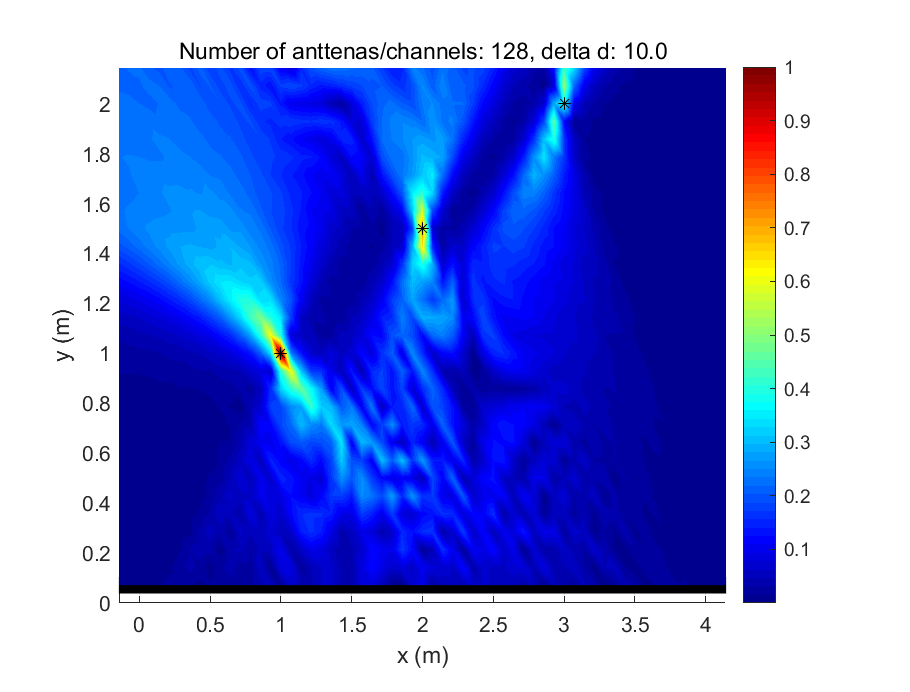
\includegraphics[width=1\textwidth]{figures/cm/N128d10.eps}
      \caption{接收机天线阵元数$N=128$,$\Delta_d = 10\text{m}$}
  \end{subfigure}
  \begin{subfigure}[t]{.45\linewidth}
      \centering
      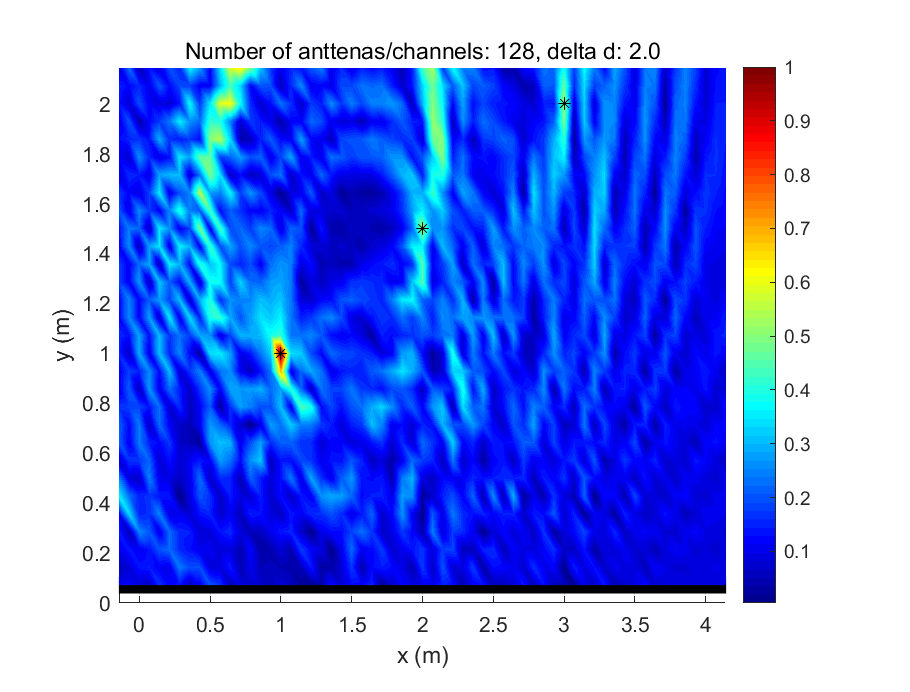
\includegraphics[width=1\textwidth]{figures/cm/N128d2.eps}
      \caption{接收机天线阵元数$N=128$,$\Delta_d = 2\text{m}$}
  \end{subfigure}
  \\
  \begin{subfigure}[t]{.45\linewidth}
    \centering
    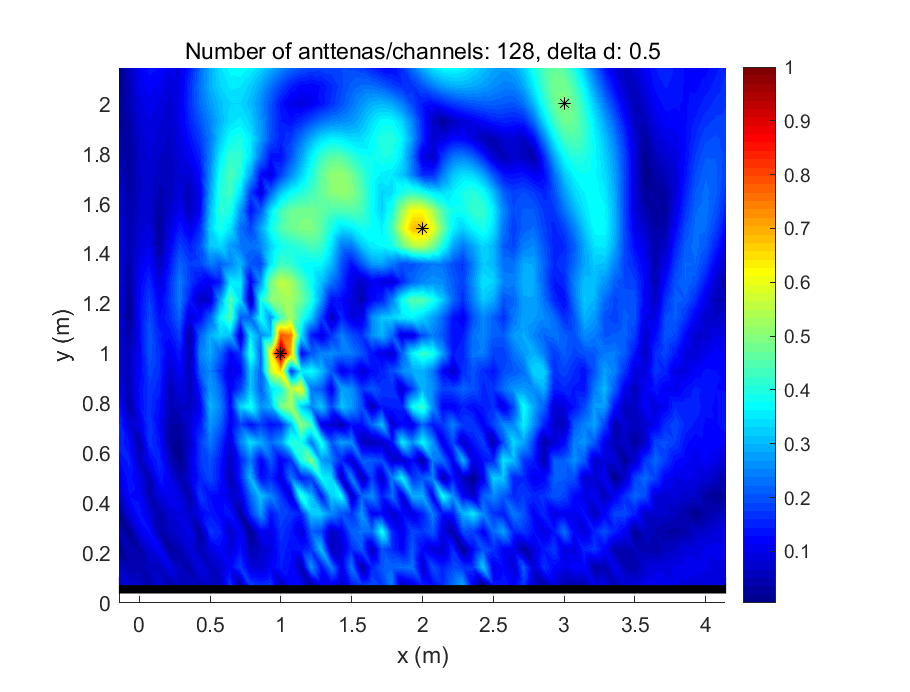
\includegraphics[width=1\textwidth]{figures/cm/N128d0.5.eps}
    \caption{接收机天线阵元数$N=128$,$\Delta_d = 0.5\text{m}$}
  \end{subfigure}
  \begin{subfigure}[t]{.45\linewidth}
    \centering
    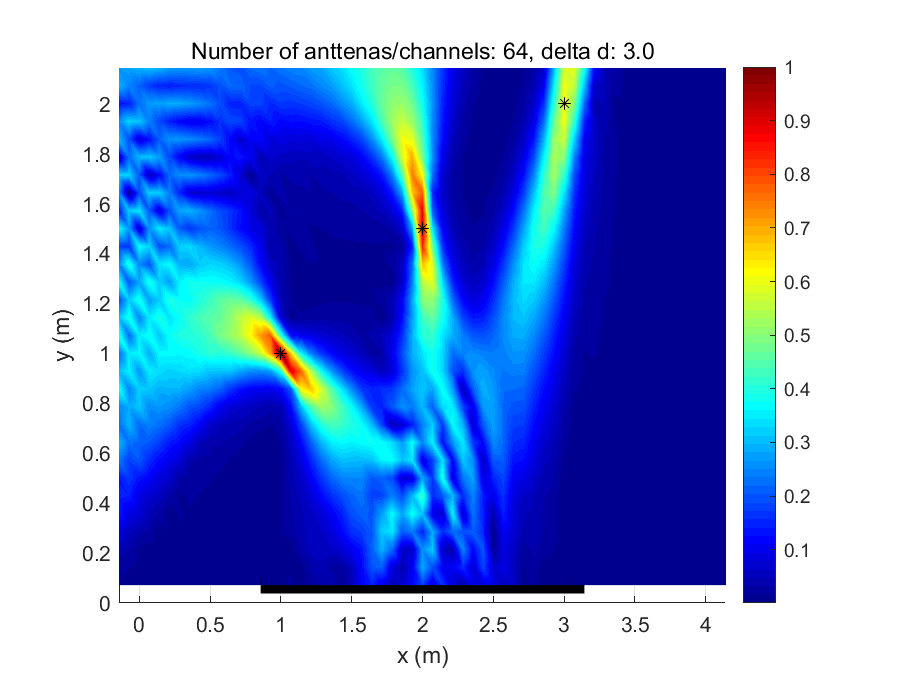
\includegraphics[width=1\textwidth]{figures/cm/N64d3.eps}
    \caption{接收机天线阵元数$N=64$,$\Delta_d = 3\text{m}$}
  \end{subfigure}
  \\
  \begin{subfigure}[t]{.45\linewidth}
    \centering
    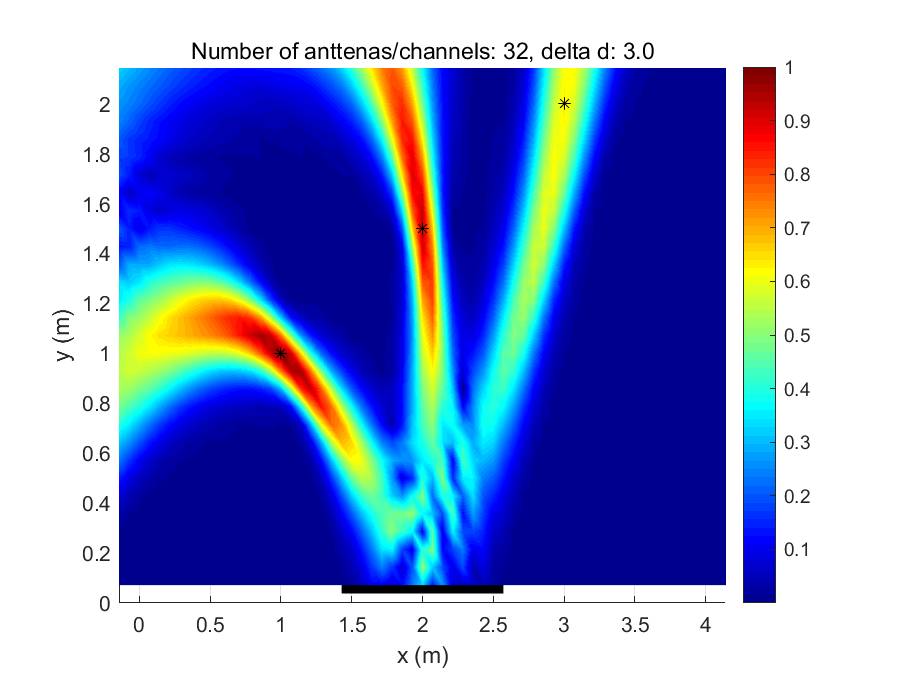
\includegraphics[width=1\textwidth]{figures/cm/N32d3.eps}
    \caption{接收机天线阵元数$N=32$,$\Delta_d = 3\text{m}$}
  \end{subfigure}
  \caption{共轭相乘消除频偏成像结果}\label{共轭相乘消除频偏成像结果}
\end{figure}


图~\ref{结合PARAFAC算法与共轭相乘消除频偏成像仿真结果}展示了结合PARAFAC算法与共轭相乘消除频偏成像仿真结果:
\begin{figure}[H]
  \centering
  \begin{subfigure}[t]{.45\linewidth}
      \centering
      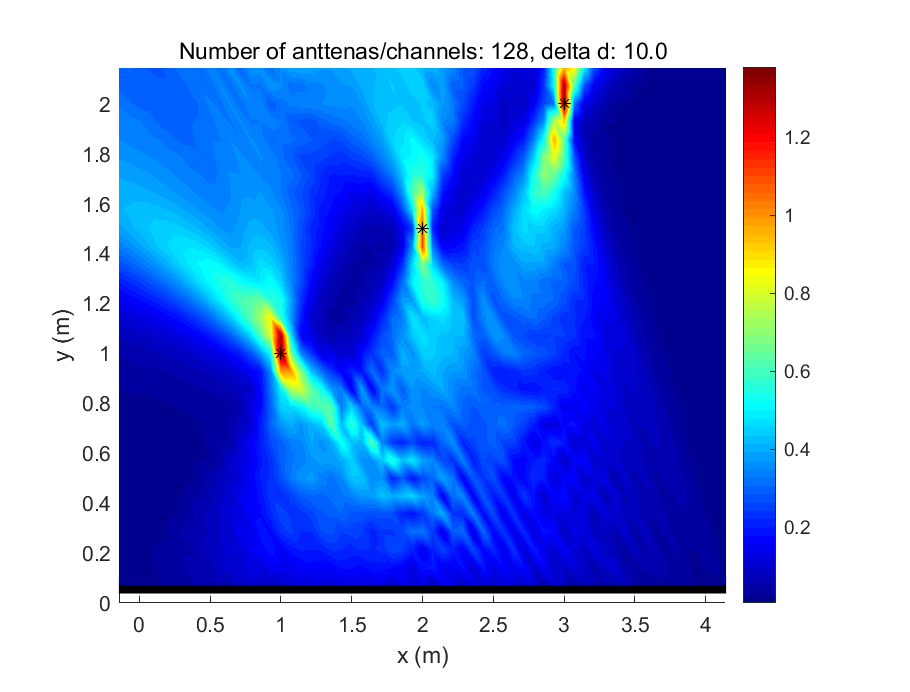
\includegraphics[width=1\textwidth]{figures/TPF/N128d10.eps}
      \caption{接收机天线阵元数$N=128$,$\Delta_d = 10\text{m}$}
  \end{subfigure}
  \begin{subfigure}[t]{.45\linewidth}
      \centering
      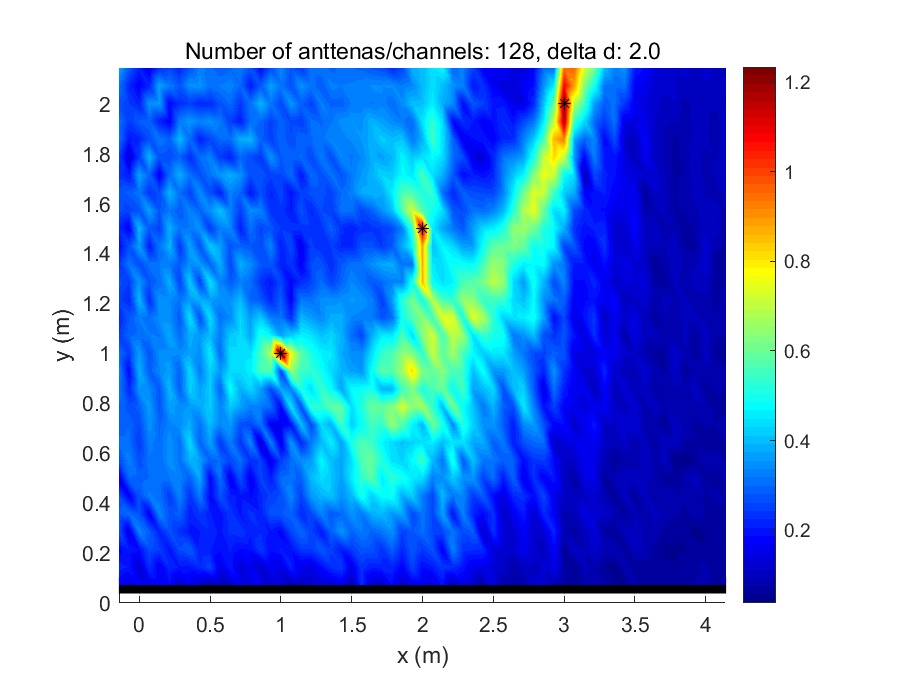
\includegraphics[width=1\textwidth]{figures/TPF/N128d2.eps}
      \caption{接收机天线阵元数$N=128$,$\Delta_d = 2\text{m}$}
  \end{subfigure}
  \\
  \begin{subfigure}[t]{.45\linewidth}
    \centering
    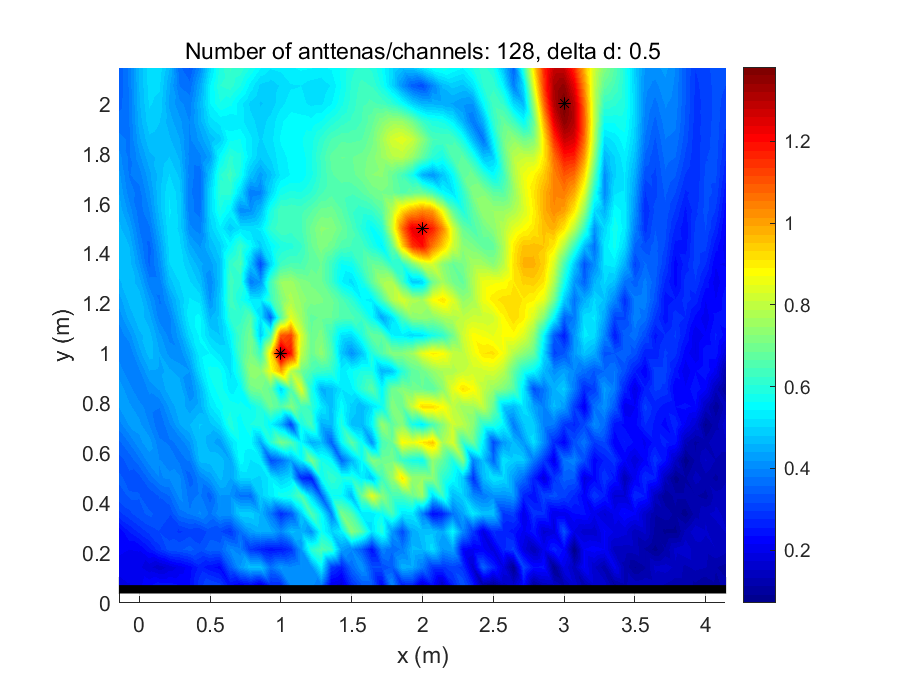
\includegraphics[width=1\textwidth]{figures/TPF/N128d0.5.eps}
    \caption{接收机天线阵元数$N=128$,$\Delta_d = 0.5\text{m}$}
  \end{subfigure}
  \begin{subfigure}[t]{.45\linewidth}
    \centering
    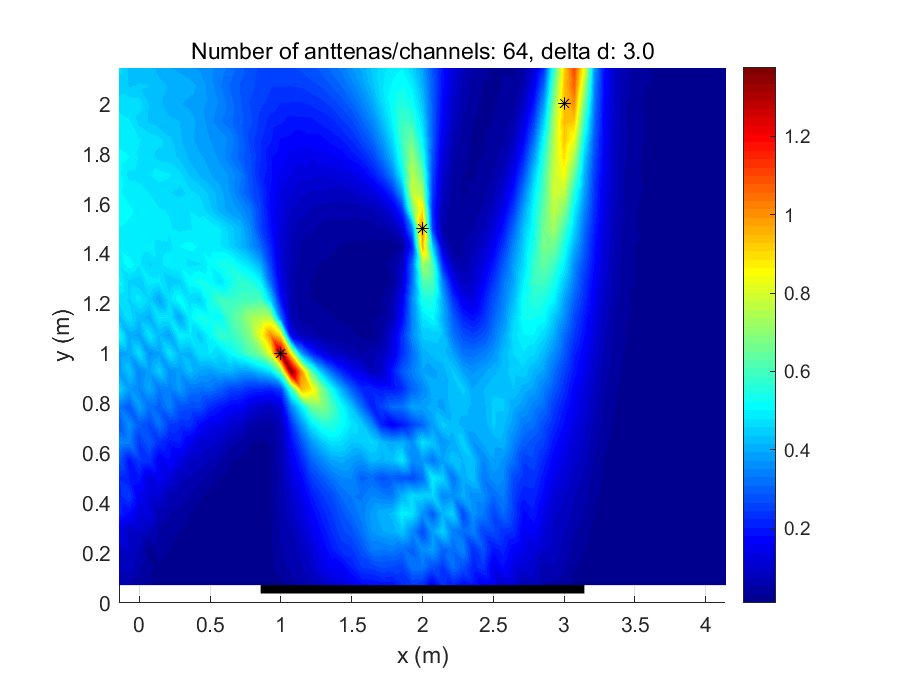
\includegraphics[width=1\textwidth]{figures/TPF/N64d3.eps}
    \caption{接收机天线阵元数$N=64$,$\Delta_d = 3\text{m}$}
  \end{subfigure}
  \\
  \begin{subfigure}[t]{.45\linewidth}
    \centering
    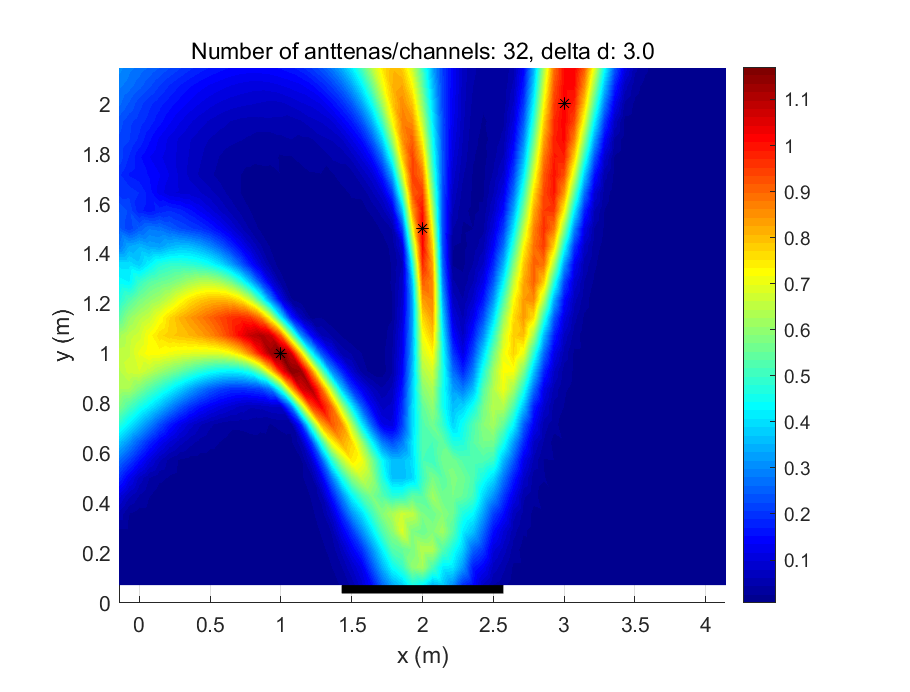
\includegraphics[width=1\textwidth]{figures/TPF/N32d3.eps}
    \caption{接收机天线阵元数$N=32$,$\Delta_d = 3\text{m}$}
  \end{subfigure}
  \caption{结合PARAFAC算法与共轭相乘消除频偏成像仿真结果}\label{结合PARAFAC算法与共轭相乘消除频偏成像仿真结果}
\end{figure}


将图~\ref{共轭相乘消除频偏成像结果}与图~\ref{结合PARAFAC算法与共轭相乘消除频偏成像仿真结果}对比,可以看出
结合PARAFAC的共轭相乘消除频偏的成像具有更加明显的峰值,但是都需要一个大的天线阵列,以及一个较大的两路天线阵列的间隔。


为了更好的展示成像的差别,根据表~\ref{对比},我们在接收天线数量$N=32$的情形下,考虑公式\eqref{情形一},\eqref{情形二}两种频偏模型,
对不消除频偏直接成像,不消除频偏并利用PARAFAC算法增强峰值直接成像,共轭相乘消除频偏成像,结合CSI共轭相乘和PARAFAC算法消除频偏等
四种成像进行了对比,见图~\ref{成像对比图}。可以看出,自发自收与情形二的仿真结果一致,说明如果我们有一个足够长的天线阵列,则不需要频偏消除。
PARAFAC算法可以有效增强峰值,但目前在情形一仍然不能太好的处理频偏。


\begin{figure}[H]
  \centering
  \begin{subfigure}[t]{.3\linewidth}
    \centering
    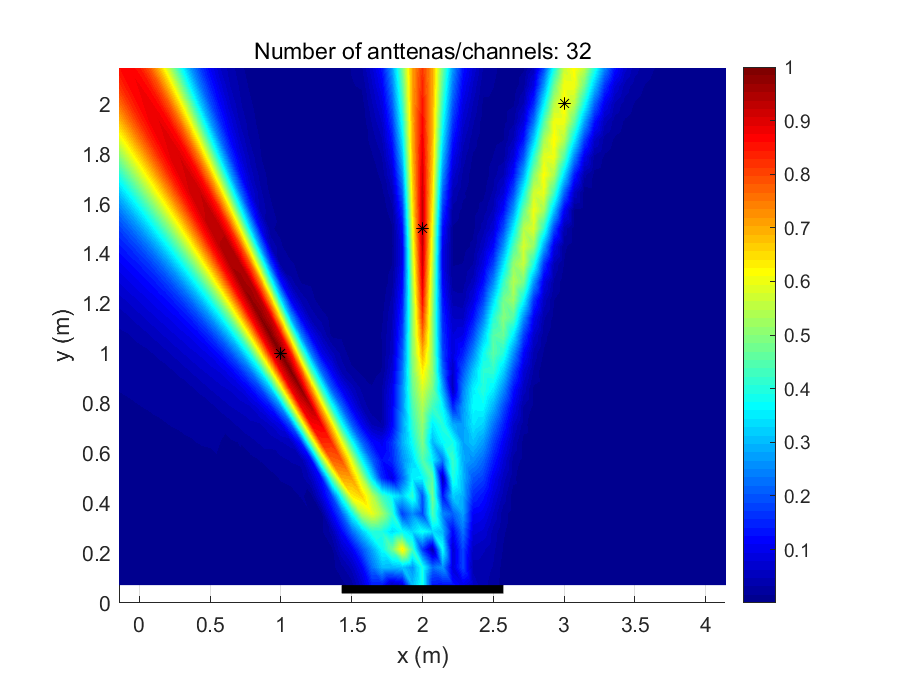
\includegraphics[width=1\textwidth]{figures/compare/CSI_without_freq.eps}
    \caption{未添加频偏~直接成像}
  \end{subfigure}
  \begin{subfigure}[t]{.3\linewidth}
    \centering
    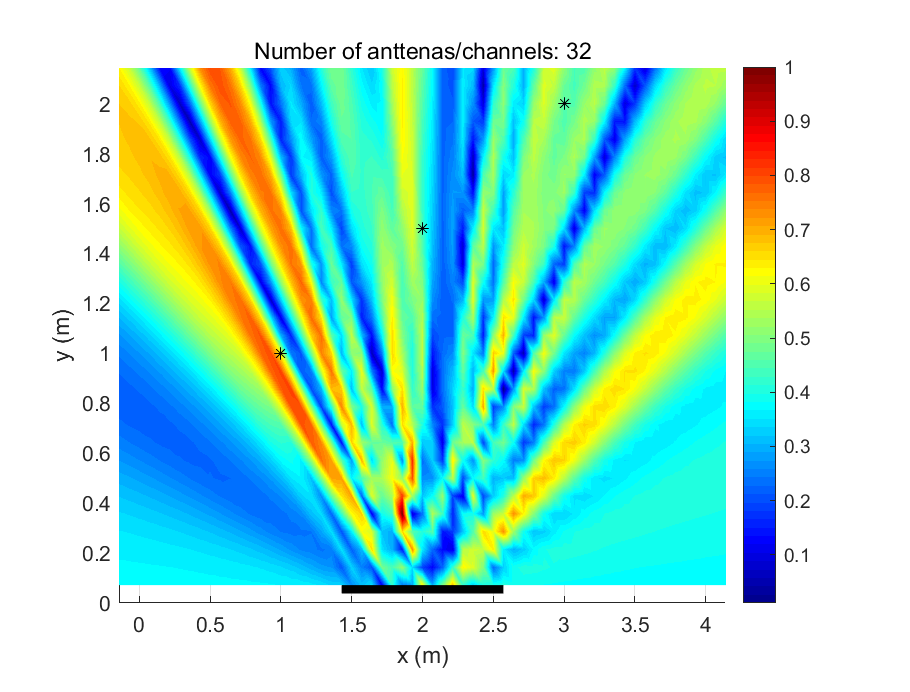
\includegraphics[width=1\textwidth]{figures/compare/CSI_freq1.eps}
    \caption{情形一频偏~直接成像}
  \end{subfigure}
  \begin{subfigure}[t]{.3\linewidth}
    \centering
    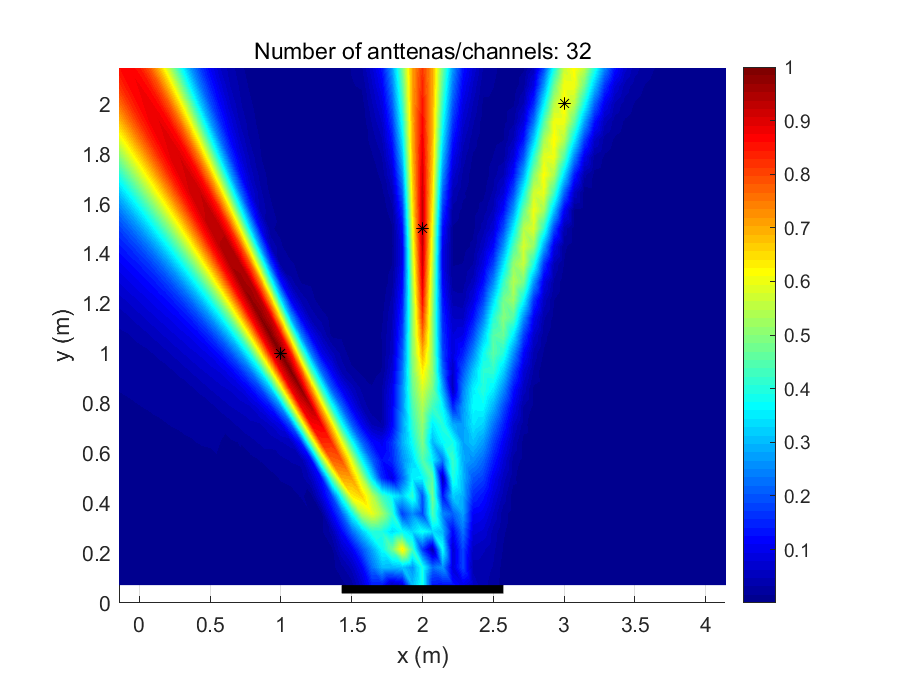
\includegraphics[width=1\textwidth]{figures/compare/CSI_freq2.eps}
    \caption{情形二频偏~直接成像}
  \end{subfigure}
  \\
  \begin{subfigure}[t]{.3\linewidth}
    \centering
    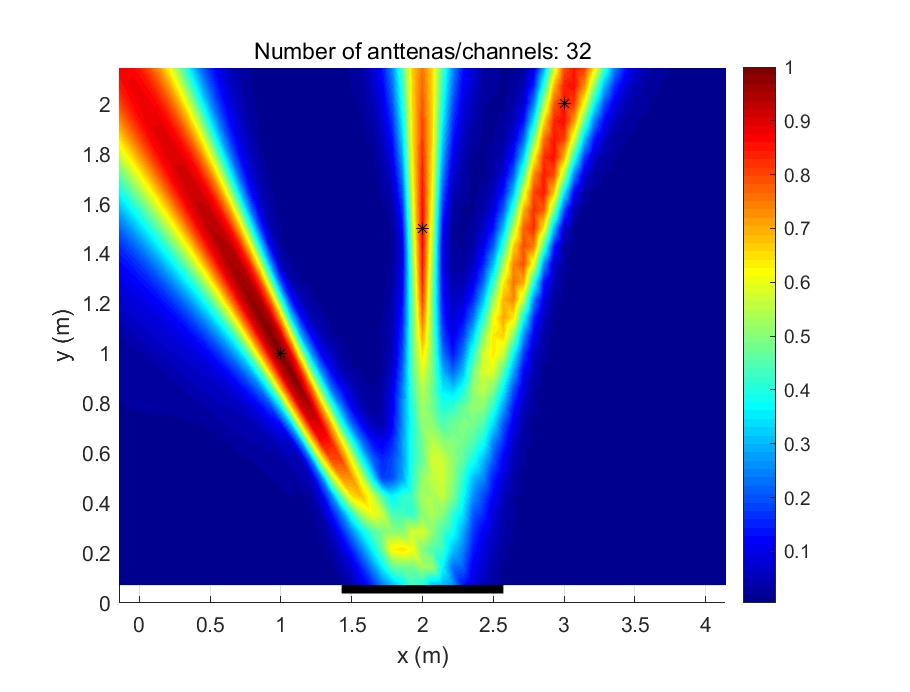
\includegraphics[width=1\textwidth]{figures/compare/TPF_without_freq.eps}
    \caption{未添加频偏~PARAFAC成像}
  \end{subfigure}
  \begin{subfigure}[t]{.3\linewidth}
    \centering
    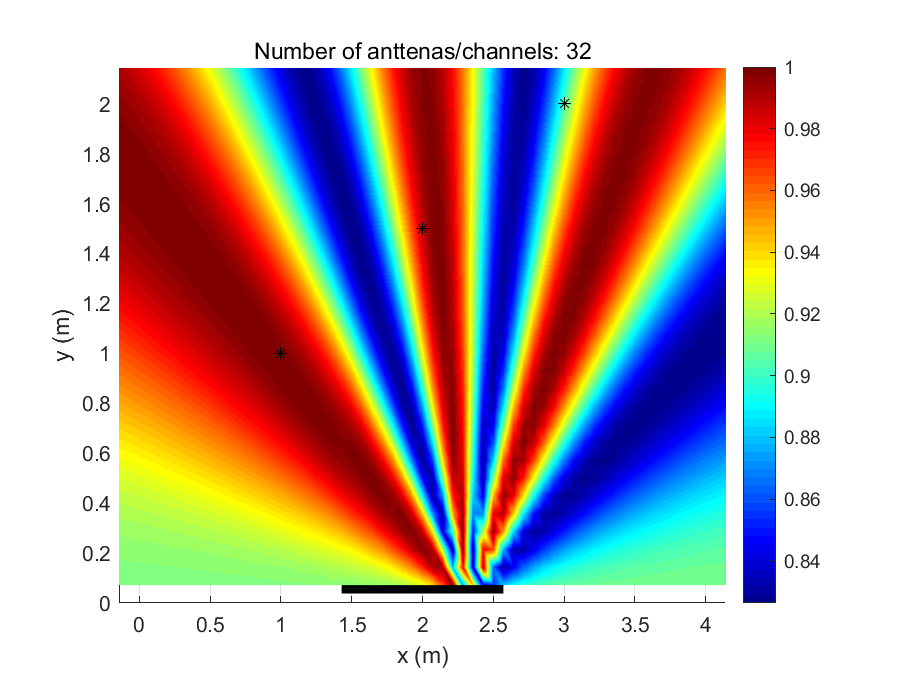
\includegraphics[width=1\textwidth]{figures/compare/TPF_freq1.eps}
    \caption{情形一频偏~PARAFAC成像}
  \end{subfigure}
  \begin{subfigure}[t]{.3\linewidth}
    \centering
    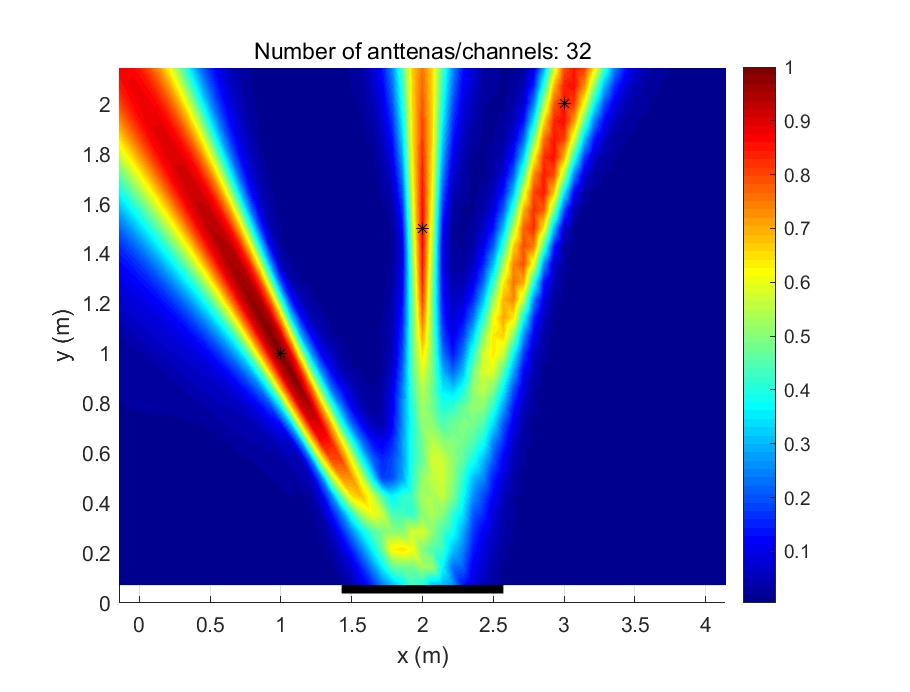
\includegraphics[width=1\textwidth]{figures/compare/TPF_freq2.eps}
    \caption{情形一频偏~PARAFAC成像}
  \end{subfigure}
  \\
  \begin{subfigure}[t]{.3\linewidth}
    \centering
    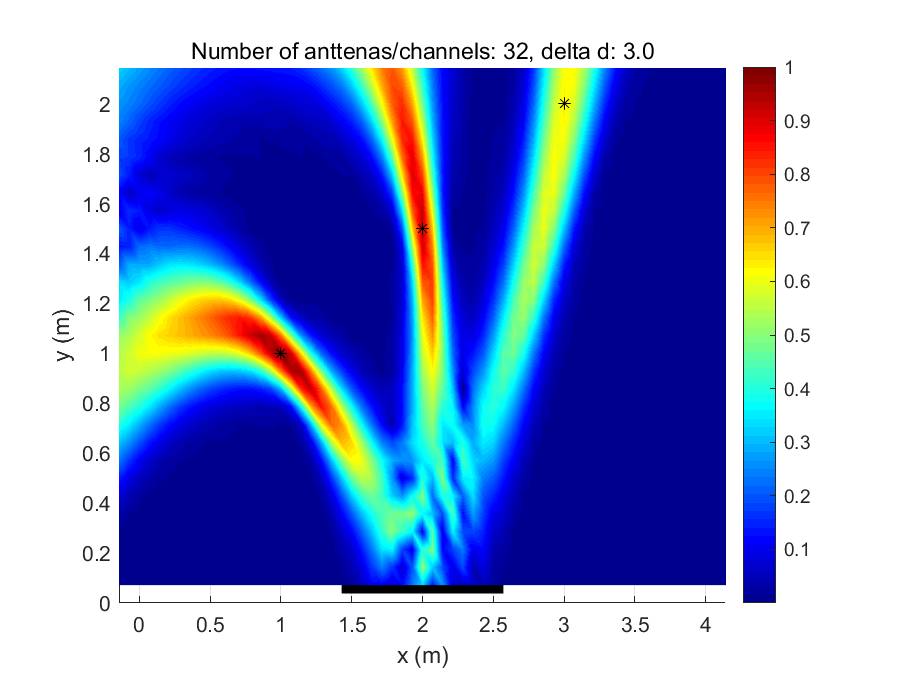
\includegraphics[width=1\textwidth]{figures/compare/CM_without_freq.eps}
    \caption{未添加频偏~共轭相乘成像}
  \end{subfigure}
  \begin{subfigure}[t]{.3\linewidth}
    \centering
    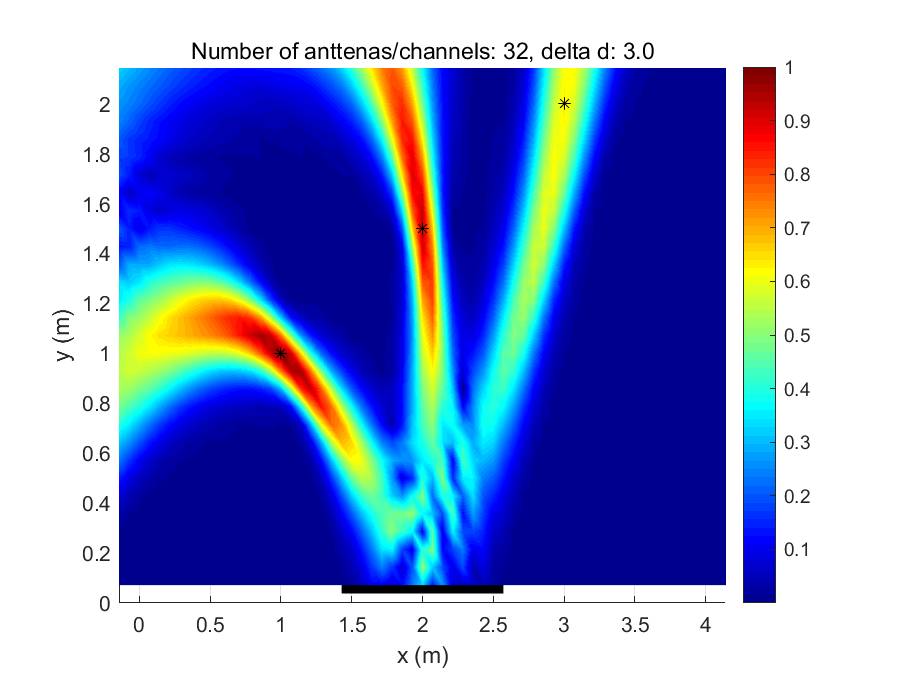
\includegraphics[width=1\textwidth]{figures/compare/CM_freq1.eps}
    \caption{情形一频偏~共轭相乘成像}
  \end{subfigure}
  \begin{subfigure}[t]{.3\linewidth}
    \centering
    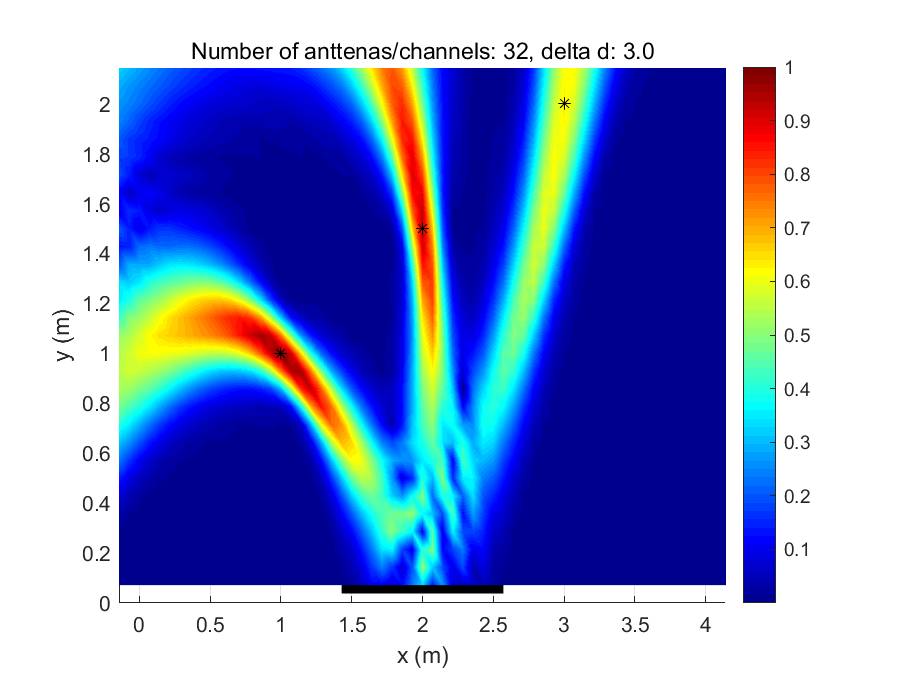
\includegraphics[width=1\textwidth]{figures/compare/CM_freq2.eps}
    \caption{情形二频偏~共轭相乘成像}
  \end{subfigure}
  \\
  \begin{subfigure}[t]{.3\linewidth}
    \centering
    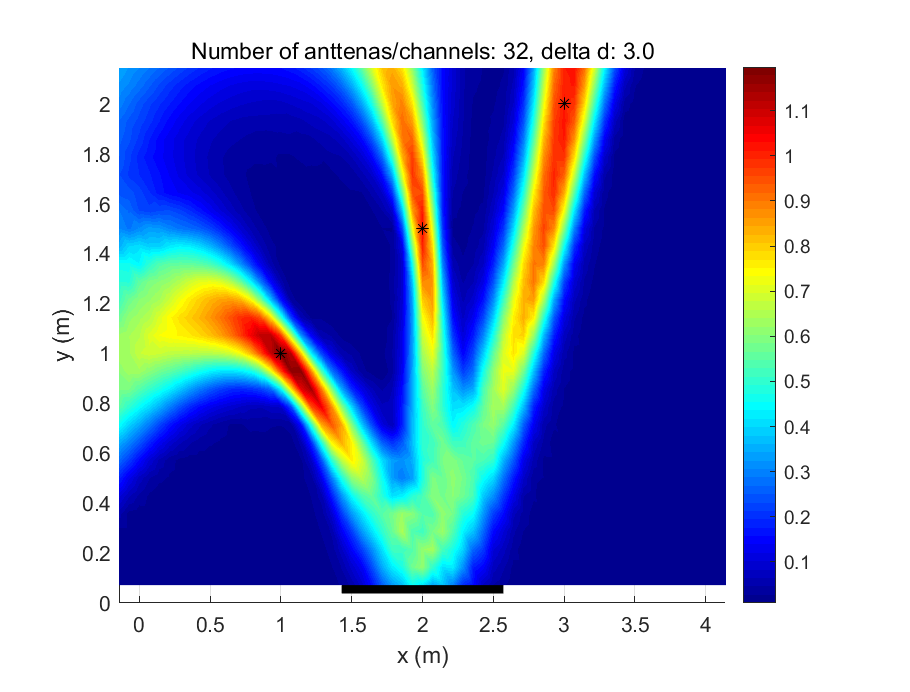
\includegraphics[width=1\textwidth]{figures/compare/TPF_CM_without_freq.eps}
    \caption{未添加频偏~结合PARAFAC与共轭相乘成像}
  \end{subfigure}
  \begin{subfigure}[t]{.3\linewidth}
    \centering
    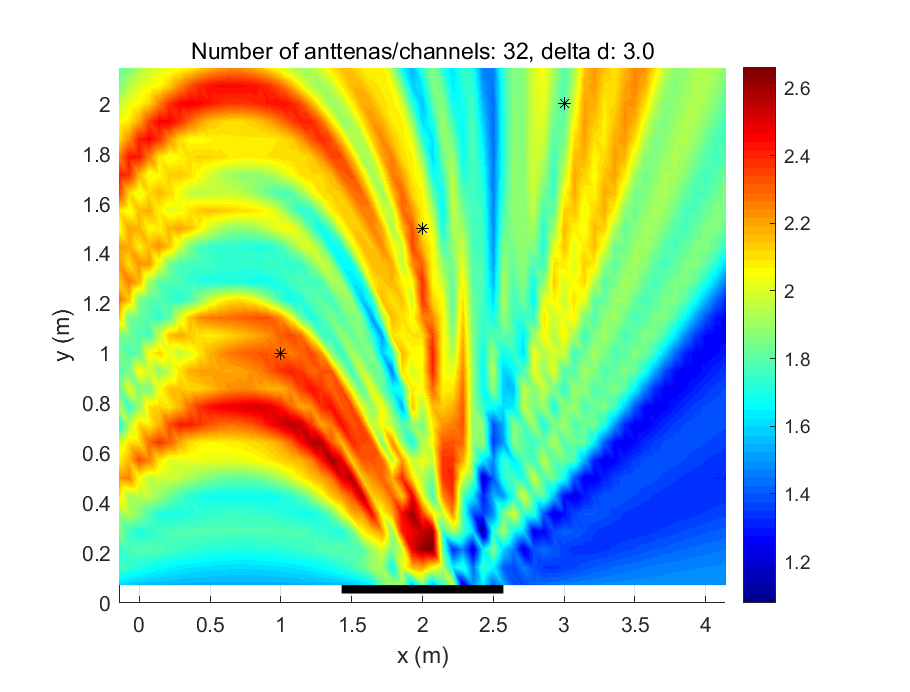
\includegraphics[width=1\textwidth]{figures/compare/TPF_CM_freq1.eps}
    \caption{情形一频偏~结合PARAFAC与共轭相乘成像}
  \end{subfigure}
  \begin{subfigure}[t]{.3\linewidth}
    \centering
    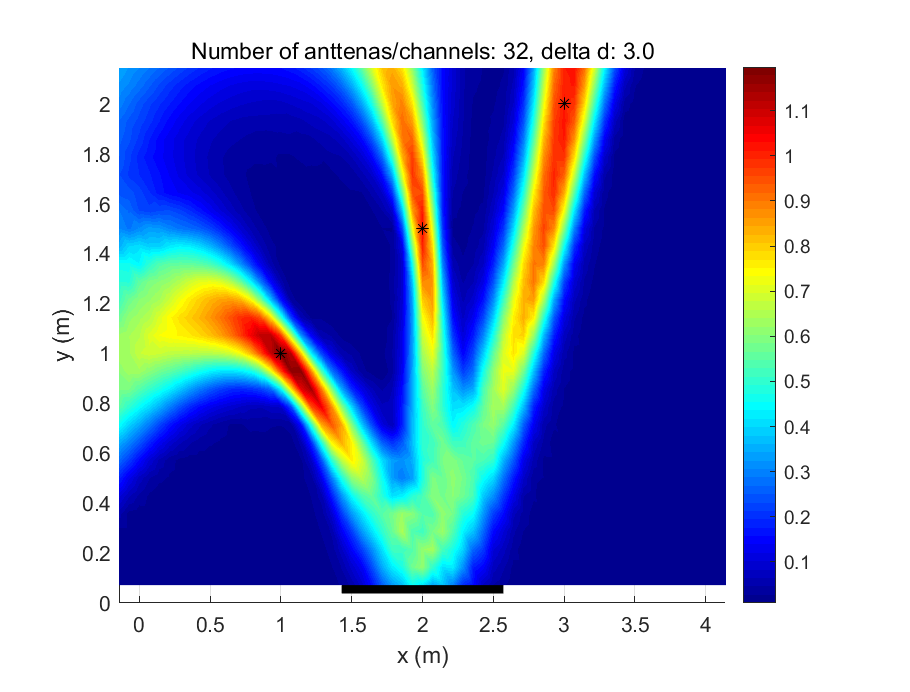
\includegraphics[width=1\textwidth]{figures/compare/TPF_CM_freq2.eps}
    \caption{情形二频偏~结合PARAFAC与共轭相乘成像}
  \end{subfigure}
  \caption{成像各种情况对比}\label{成像对比图}
\end{figure}